\documentclass{eniepaper}
\卒論
%\修論
\usepackage{epsbox}
\usepackage{makeidx}
\usepackage{fancybox}
\usepackage{subfloat}
\usepackage[dvips]{graphicx}
  \title {卒業論文及び修士論文を書くにあたって}         
   \author{佐野 裕也}   
   \teacher{香川~考司} 
   \year{平成29年度~(2017年度)}              
\date{平成29年2月00日}                               
% \date{\today}
                                                          
\makeindex                                                
                                         
\etitle{This is the English Title.}
% 2006/2/7改訂
% タイトルを複数行にしたいときは、下のetitleenv環境を使ってください。
%\begin{etitleenv}
%This is 
%the very very very very very very very very very very very very long long long English Title.
%\end{etitleenv}

\begin{eabstract}
This is the abstract.
This is the abstract.
This is the abstract.
This is the abstract.
This is the abstract.
This is the abstract.
This is the abstract.
This is the abstract.
This is the abstract.
This is the abstract.
This is the abstract.
This is the abstract.
This is the abstract.
This is the abstract.
This is the abstract.
This is the abstract.
This is the abstract.
This is the abstract.
This is the abstract.
This is the abstract.
This is the abstract.
This is the abstract.
This is the abstract.
This is the abstract.
This is the abstract.
\end{eabstract}

\begin{jabstract}
プログラミング初心者が新たなプログラミング言語を学習するとき、プログラミングの基礎概念
と言語の文法を同時に学習しなければならない。 これは、 学習者にとって大き
な負担である。これを解決するために尾崎の研究では、Webベースグラフィカル
プログラミングエディタであるBlocklyをC言語に対応させた。また山形の研究では、
Blocklyに練習問題を提示する機能を実装した。本研究では、Blocklyを多言語対応し、
ブロックの動的変形の機能を増やして、プログラミング初心者の学習の幅を広げることを
目的としている。
\end{jabstract}


\begin{keyword}
プログラミング学習, C言語, JavaScript, Haskell, Flex, Webベース
\end{keyword}

\begin{document} 
\maketitle
%  \listoffigures % 図の目次
%  \listoftables  % 表の目次
                                                          
   \chapter{はじめに}
   
   \section{はじめに}


  プログラミング学習者は、以下の2つを同時に学ばなければならない。
  
\begin{itemize}
\item プログラミングの基礎概念
\item 各プログラミング言語の文法
\end{itemize} 

 これらを学ぶことは、学習者にとって大きな負担である。
 この負担を軽減するために、文法を意識せずにプログラミングができる学習環境が必要である。これを解決するために、Webベースのビジュアルプログラミング言語であるBlocklyを用いる。
  
Blocklyとは、Googleで開発されているグラフィカルなプログラミングエディタである。図1のようなブロックを繋ぎ合せることでプログラミングを行う。このため構文エラーに悩まされず、直感的にプログラミングをすることができる。JavaScriptで記述されており、ドキュメントも豊富に用意されているためカスタマイズが容易である。また、BlocklyはWebベースのアプリケーションであるため、導入の作業が不要である。さらに、Blocklyで作成したプログラムは、JavaScript、 Dart、 Python、 Lua、 PHPの5種類のコードに変換して出力することができる。

\newpage
 
尾崎の研究は、BlocklyをC言語、Flex言語に対応させたもので、システムの対象者がプログラミング入門者である。このシステムによって文法を意識せずにプログラミンングを学ぶことができる。しかし、大学の講義で学習する言語に対応しきれていない。システム自体が便利であっても、大学の講義で学習する言語に対応していないと、大学生はこのシステムを利用することができない。また、ブロックの形を動的に変形することができないため、柔軟性のあるプログラミング言語をブロックの形状によって制約されてしまうことになる。尾崎の研究で実装したシステムのイメージを図\ref{fig:ozaki}に示す。
 
本研究ではBlocklyの多言語化を目標とする。多言語化によって、よりBlocklyで学習支援できる範囲が広がり、学習者が自分に適した言語を選ぶことができる。しかし、必要となるブロックの種類や形状は増加するので、ブロックの形を動的に変形させることも考えなければならない。 
\\
\\
\\
\\
\\
\begin{figure}[h]
\begin{center}
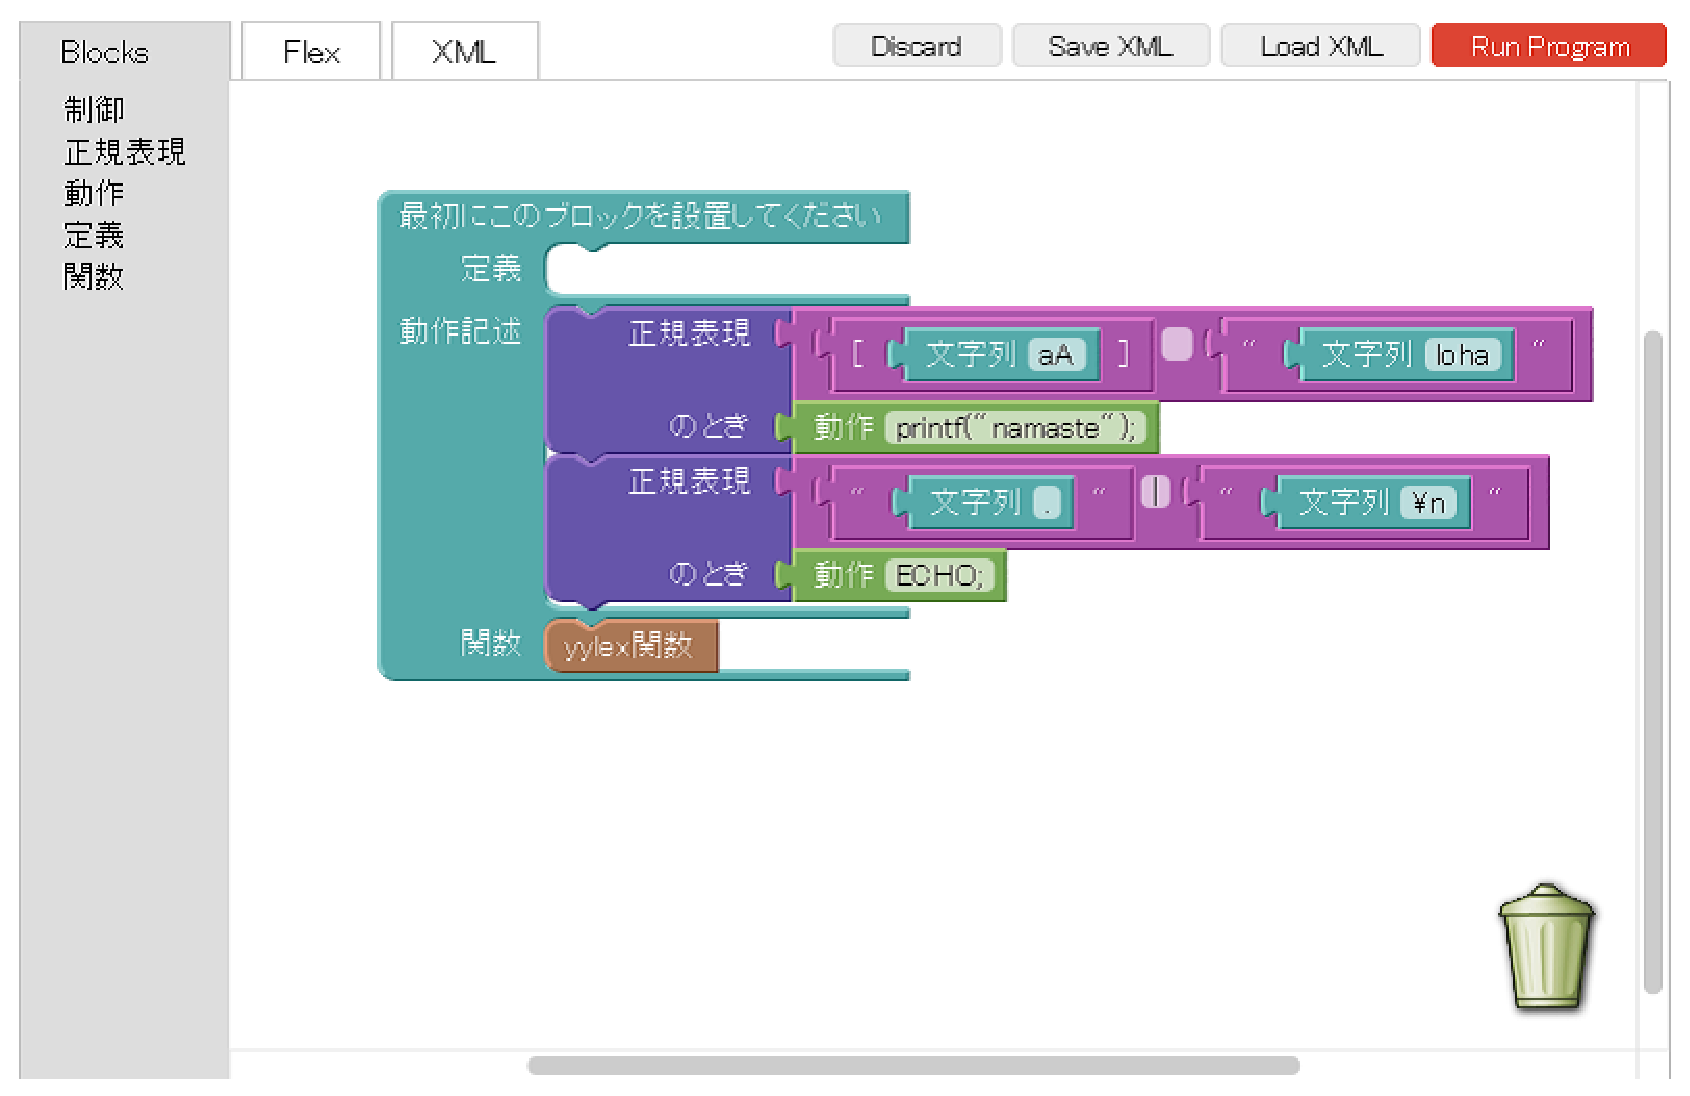
\includegraphics[scale=0.3]{img/ozaki.eps}
\caption{尾崎の研究で実装したシステム}%
\label{fig:ozaki}
\end{center}%
\end{figure}% 

\newpage

   \section{Webベースの利点}
   
本研究で開発したシステムは、Webベースシステムである。Webページすることにより、学習者に次のような利点があると考えられる。

\begin{itemize}
\item システムのインストールが不要
\item Webブラウザがあるば実現可能
\item 常に最新版のシステムが可能
\end{itemize} 

また、教員側にも次のような利点がある。

\begin{itemize}
\item システムのカスタマイズが容易
\item システムの不具合をすぐに修正可能
\item 導入に関する指導が不要
\end{itemize} 

サーバ側にアプリケーションを設置することで、クライアント側ではアプリケーションを導入する必要がなく、Webブラウザがあれば学習者にとって、簡単にそして常に最新のシステムが利用可能である。教員にとってもシステムのカスタマイズが容易で、不具合もすぐに修正できるので、システムの運営がとてもやりやすくなる。
 
 \newpage
 
    \section{システムに求められる要件}
    
先行研究の問題点より、本システムに求められる要件は以下の3つである。
 
\begin{itemize}
\item プログラミング学習者の負担を軽減させる
\item 大学の講義で学習する言語に対応させるための多言語化
\item ブロックの動的変形を拡張
\end{itemize} 

既存のBlocklyの対応言語が、大学の講義で学習する言語に対応しきれていないという問題点を踏まえて、システムの多言語化が必要である。
システムの多言語を行うことで必要となるブロックの種類が増加する。
また、柔軟性のあるプログラミング言語をブロックの形状によって制約されてしまう。
これらに対応するために、ブロックの動的変形機能を拡張する。
その際に、プログラミング学習者の負担を軽減させることが目的なので、拡張する機能を複雑にしてはいけない。

本論文では、第2章でBlocklyについて、第3章で実装したシステム、第4章でシステムの評価、第5章でまとめ、今後の課題について述べる。



   \chapter{Blockly}
   
   \section{全体の主なファイル構成}
   
\begin{itemize}

\item Library フォルダ

システム自体の定義を行うプログラムで構成されている。
また、blocklyフォルダには、Blocklyの本体であるblockly\_compressed.jsファイルが存在する。
いずれもGoogleが用意した元からあるファイルである。

\item js フォルダ

こちらもシステム自体の定義を行うプログラムで構成されている。
システムの拡張を行いたい場合はこちらから行う。

\item MyBlock フォルダ

このフォルダの直下にブロックの種類ごとのファイルがあり、ブロックの形状を定義している。
いずれもGoogleが用意した元からあるファイルであり、これらのプログラムはビルドされ、
Libraryフォルダのblocks\_compressed.jsファイルに圧縮されている。
そのため、これらのファイルを書き換えてもシステムが変更されることはない。

\item MyBlock2 フォルダ

このフォルダの直下にブロックの種類ごとのファイルがあり、こちらもブロックの形状を定義している。
このフォルダの中のファイルは私自身が作成したもので、新たなブロックを定義したり、
ブロックの形状を変更したいときはこちらにプログラムを記述する。

  \newpage

\item Mygenerators フォルダ

このフォルダの直下に各プログラミング言語のフォルダがある。
それらのフォルダの中にブロックの種類ごとのファイルがあり、各ブロックを配置したときに出力されるソースコードの内容が書かれている。

\item html フォルダ

Webページの仕様を定義するプログラムで構成されている。

\item index.html ファイル

私が作成したデモページのホーム画面の仕様を定義しているファイルである。



\item デモページのファイル群

\shadowbox{
\begin{minipage}[t]{6cm}
\begin{verbatim}
c.html
javascript.html
Haskell.html
Flex.html
\end{verbatim}
\end{minipage}
}

これらのプログラムは、デモページを構成しいぇいるhtmlファイルである。

\end{itemize} 
   
 \newpage
  
   \section{システム構成}
   
Blocklyは、ワークスペース部、ブロックメニュー部、ソースコード部、XMLコード部の4つのコンポーネントによって構成される。図\ref{fig:Blockly}にBlocklyのイメージを示す。デフォルトでは、ワークスペース部が表示されており、ソースコードタブを押すとソースコード部のコンポーネントに切り替わり、XMLコードタブを押すとXMLコード部のコンポーネントに切り替わる。ブロックメニュー部は常に左部のに表示されている。ここでは、それぞれのコンポーネントについて説明する。
  

\begin{figure}[h]
\begin{center}
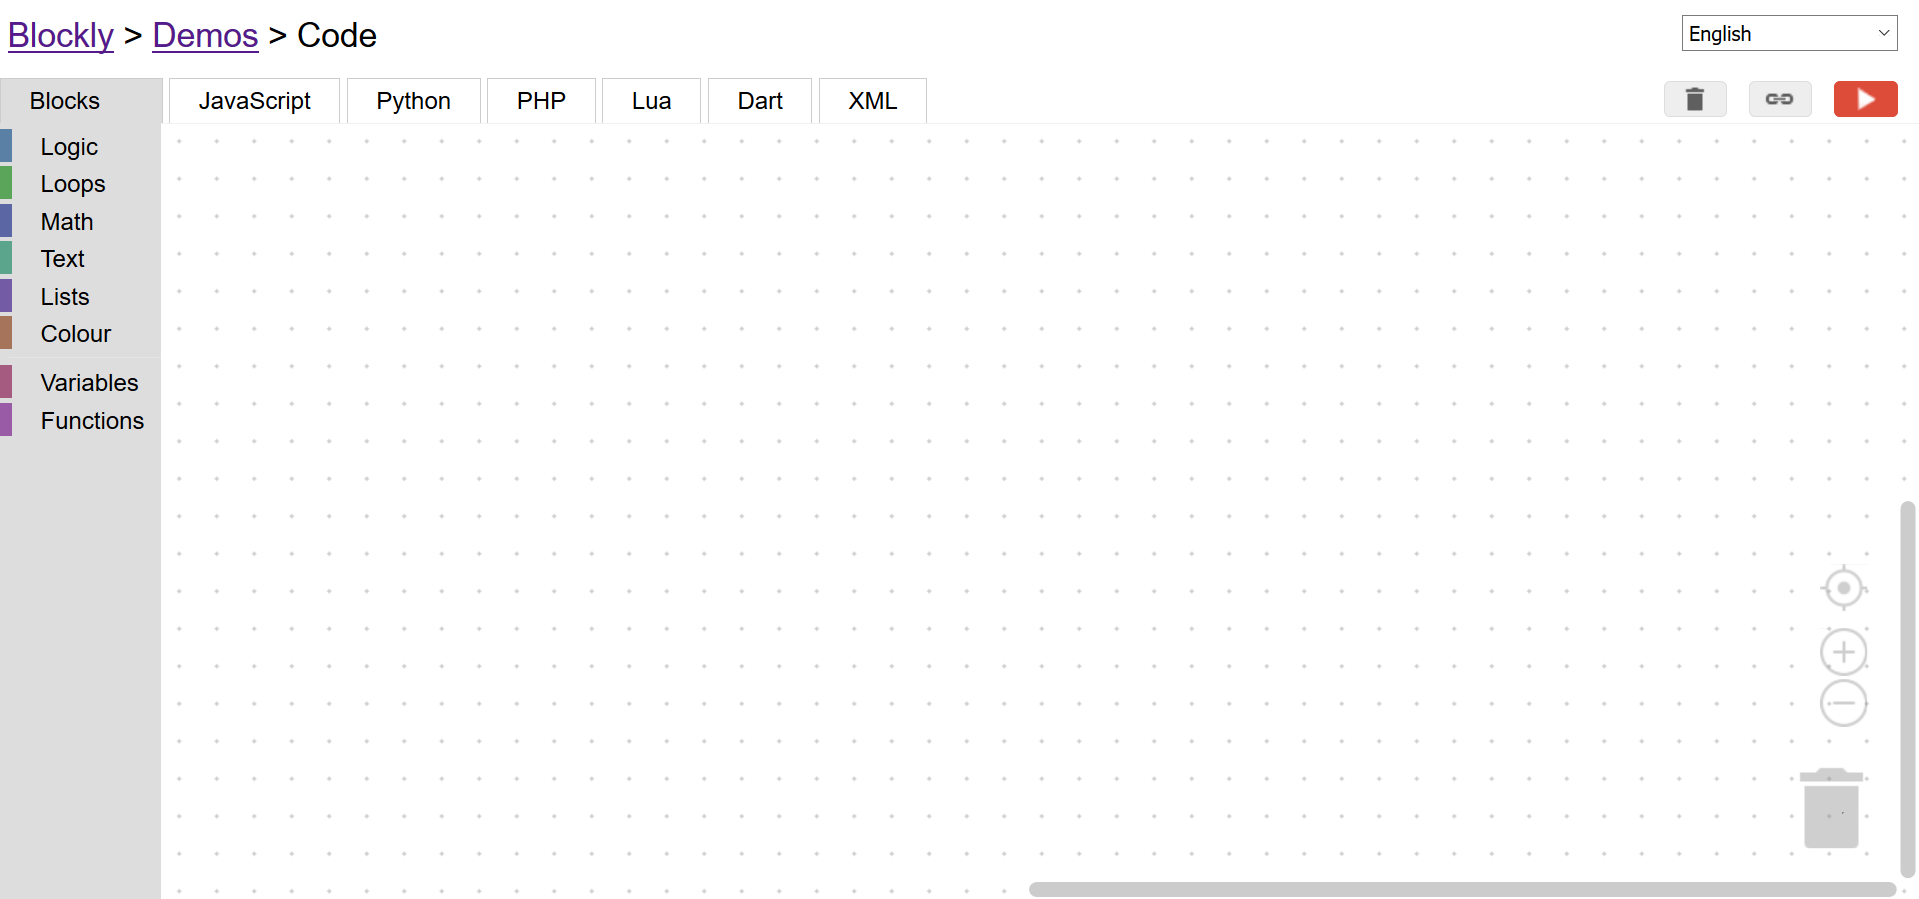
\includegraphics[scale=0.4]{img/Blockly.eps}
\caption{Blockly}%
\label{fig:Blockly}
\end{center}%
\end{figure}% 

   \newpage

   \subsection{ワークスペース部}

ワークスペース部は、ブロックを使ってプログラミングを行うスペースである。図\ref{fig:workspace}にワークスペース部のイメージを示す。ユーザは、ブロック部に存在するブロックをワークスペース部にドラッグ&ドロップで自由につなぎ合わせることでプログラミングを行う。ワークスペース部の右下にはゴミ箱アイコンが存在する。ワークスペース部に設置したブロックをこのアイコンにドラッグすると、ブロックを削除することができる。その上に拡大縮小アイコン、さらにその上に中央に寄せるアイコンが表示されている。

また、ワークスペース部に設置したブロックを右クリックすることで、以下のような動作が行える。

\begin{itemize}
\item ブロックの複製
\item コメントの追加
\item ブロックの接続表現の切り替え
\item ブロックの表現の簡略化
\item ブロックの透明化
\item ブロックの削除
\item ブロックの動作を説明するWebページを表示
\end{itemize} 
   
\begin{figure}[h]
\begin{center}
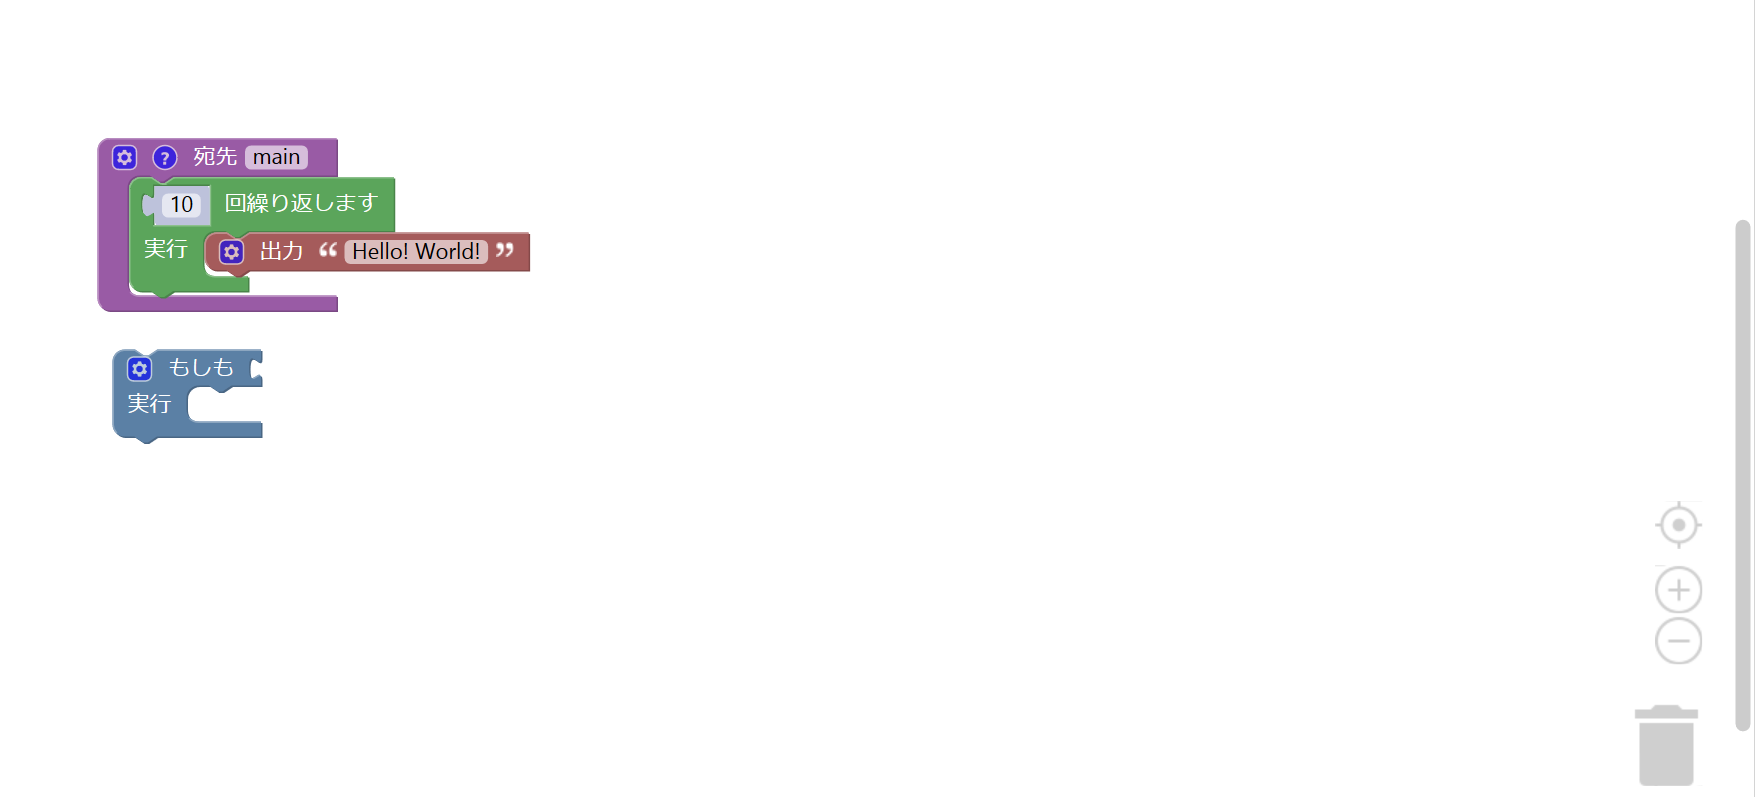
\includegraphics[scale=0.3]{img/workspace.eps}
\caption{ワークスペース部}%
\label{fig:workspace}
\end{center}%
\end{figure}% 

   \newpage

   \subsection{ブロックメニュー部}
   
ブロックメニュー部は、定義されたブロックが存在するスペースである。図\ref{fig:blockmenu}にブロックメニュー部のイメージを示す。ブロックは、論理、数、リストなどのカテゴリーにそれぞれ格納され、カテゴリーをクリックすると、そのカテゴリーに格納されたブロックが表示される。図\ref{fig:blockmenu_open}にカテゴリーをクリックしたときのイメージを示す。ユーザは、このブロックメニューから新たに必要なブロックを選択して使用する。

\begin{figure}[h]
\begin{center}
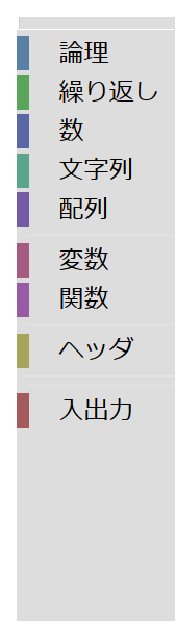
\includegraphics[scale=0.3]{img/blockmenu.eps}
\caption{ブロックメニュー部}%
\label{fig:blockmenu}
\end{center}%
\end{figure}% 

\begin{figure}[h]
\begin{center}
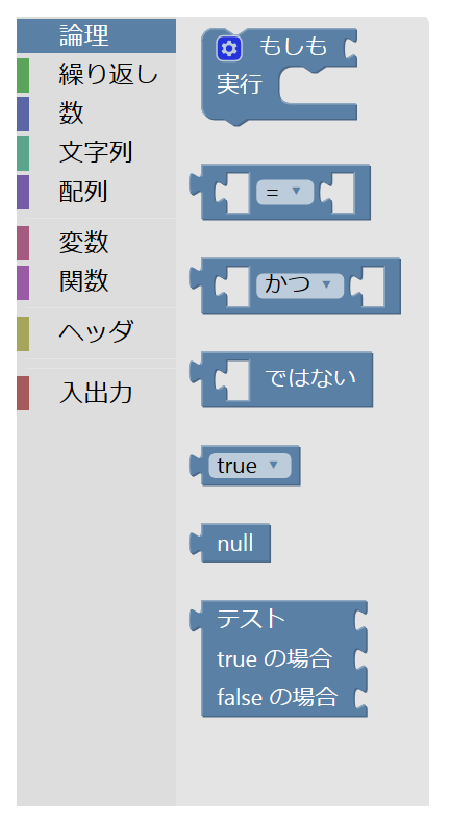
\includegraphics[scale=0.3]{img/blockmenu_open.eps}
\caption{カテゴリーをクリックしたとき}%
\label{fig:blockmenu_open}
\end{center}%
\end{figure}% 

   \newpage

   \subsection{ソースコード部}
   
ソースコード部は、作成したプログラムのソースコードを表示するスペースである。図\ref{fig:source_code}にソースコード部のイメージを示す。タブ名は各プログラミング言語の名称になる。ワークスペース部でブロックを組み合わせて作成したプログラムが、リアルタイムにソースコードに変換され、このソースコード部でいつでも確認することができる。この機能によって、Blocklyでプログラミングを学んだ学習者がソースコードを記述できるように支援する働きを持つ。システムの拡張の際に新たなブロックを実装した場合は、新たなブロックの定義と共に新たにソースコードも定義しなければならない。

\begin{figure}[h]
\begin{center}
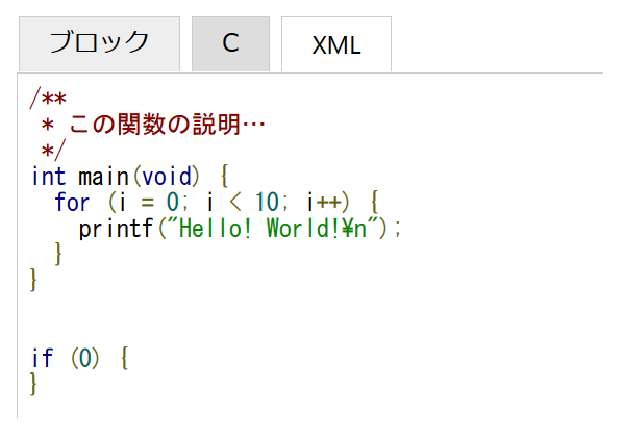
\includegraphics[scale=0.3]{img/source_code.eps}
\caption{ソースコード部}%
\label{fig:source_code}
\end{center}%
\end{figure}% 

   \subsection{XMLコード部}
   
XMLコード部は、作成したプログラムのXMLコードを表示するスペースである。図\ref{fig:XML_code}にXMLコード部のイメージを示す。ワークスペースで組み合わせたブロックの構造がXML形式で出力され、その出力されたXMLコードをセーブ、ロードすることができる。この機能によって、組み合わせたブロックを保存したり、他の学習者や教員が組み合わせたブロックを自分のワークスペース上に再現することができる。

\begin{figure}[h]
\begin{center}
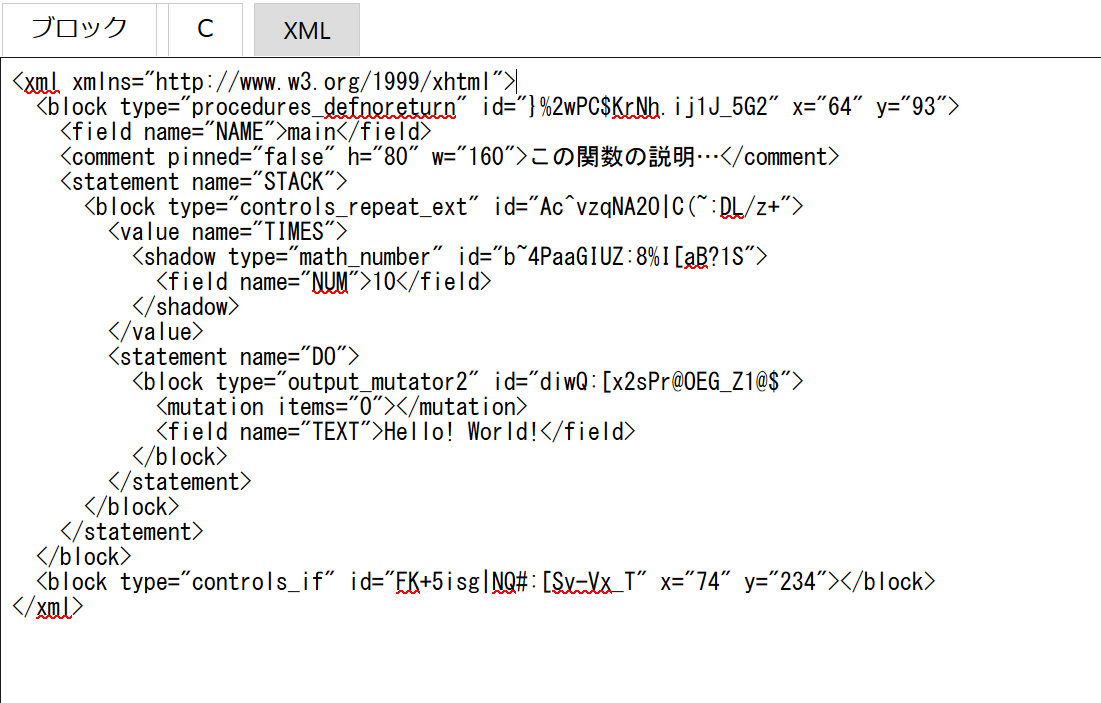
\includegraphics[scale=0.3]{img/XML_code.eps}
\caption{XMLコード部}%
\label{fig:XML_code}
\end{center}%
\end{figure}% 

   \newpage
   
   \section{Mutator機能}
   
Blocklyの機能にMutatorがある。ここでは、そのMutatorという機能について説明する。

Mutatorは、ブロックの動的変形を行う機能である。この機能は、Blocklyの用意されてる機能の中で唯一、用意されている動的変形である。図\ref{fig:mutator1}にMutatorのイメージを示す。Mutatorの機能が使えるブロックには、左上に歯車のマークがある、その歯車のマークを押すと、その近くに吹き出しの形をした小窓が現れる。小窓の左半分はブロックメニュー部、右半分はワークスペース部となっている。小窓の中のコンポーネントは、このブロック限定のものである。小窓のブロックメニュー部から拡張したいブロックを取り出し、小窓のワークスペース部の既存のブロックに取り付ける。すると、吹き出し元のブロックが変形される。図{fig:mutator2}が、そのときのイメージである。Mutator機能によって、ブロックの形をカスタマイズでき、ブロックメニュー部で用意されるブロックの種類を大幅に減らすことができる。実装で動的変形機能の拡張を行うときは、この機能を参考にして新たな動的変形機能を実装する。

\begin{figure}[h]
\begin{center}
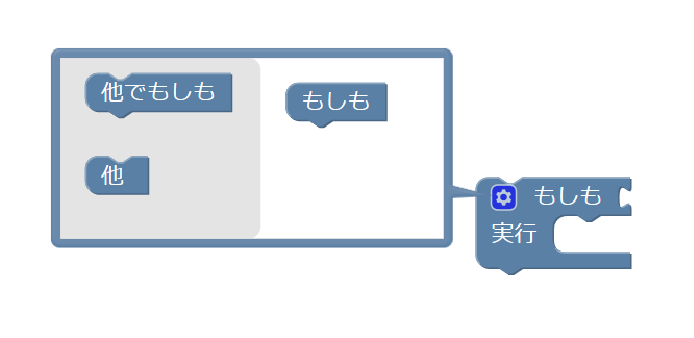
\includegraphics[scale=0.5]{img/mutator1.eps}
\caption{Mutator}%
\label{fig:mutator1}
\end{center}%
\end{figure}% 

\begin{figure}[h]
\begin{center}
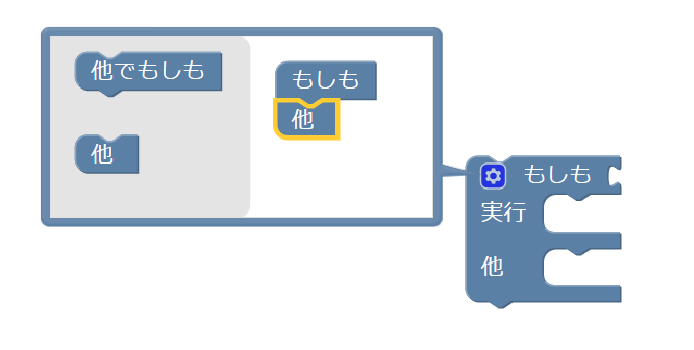
\includegraphics[scale=0.5]{img/mutator2.eps}
\caption{Mutator}%
\label{fig:mutator2}
\end{center}%
\end{figure}% 

   \chapter{実装}
   
   \section{動的変形機能}   
   
   \section{新たに作成したブロック}

   \subsection{入出力ブロック}
   
   \subsection{Blockly for C}
   
   \subsection{Blockly for Flex}
  
   \subsection{Blockly for Haskell}

   \section{サンプルボタン機能}
   
   序論を書いてください。\newpage

   文字だけで埋めるとこのような感じになります。

   \noindent
   123456789012345678901234567890123
   456789012345678901234567890123456
   789012345678901234567890123456789
   0123456789012345678901234567890123
   456789012345678901234567890123456
   789012345678901234567890123456789
   0
   
   \chapter{評価}
   
   \section{評価項目}
   
   \section{結果}
   
   序論を書いてください。
   
   \newpage

   文字だけで埋めるとこのような感じになります。

   \noindent
   123456789012345678901234567890123
   456789012345678901234567890123456
   789012345678901234567890123456789
   0123456789012345678901234567890123
   456789012345678901234567890123456
   789012345678901234567890123456789
   0

   \chapter{おわりに}
   
   \section{まとめ}
   
大学の講義で学習する言語に対応させるために、WebベースグラフィカルプログラミングエディタBlocklyの多言語対応を行った。その際に、ブロックの種類が多くなりすぎないようにMutator以外の動的変形の機能の拡張も行った。この拡張によって、柔軟性のあるプログラミンング言語をブロックの形状によって制限されないようになっている。また、拡張した機能もシンプルで、学習者の負担も増やさないようにしている。これらの特徴は、第1章で述べたシステムに求められる要件を満たしているといえる。

本研究で実装したシステムのイメージを図{fig:}に示す。
   
   \section{今後の課題}
   
   序論を書いてください。\newpage

   \section{ビジュアルプログラミング言語 Processing}
   
こちらもBlocklyと同様に、グラフィック系に特化しており、プログラミング初心者に扱いやすいものとなっている。
 ブロックのような視覚的なものでプログラミング行い、随時ソースコードと実行結果が出力されるようになっている。
 ソースコードの文法は、Javaと非常に似た独自の文法を採用している。
 学習者の対象がアート系のプログラミング初心者で、Blocklyよりも学習者のターゲットが狭い。
 
 このシステムの特徴として、ライブプログラミングという機能を導入している。
 通常ならば、①プログラムを書く ②コンパイルする ③実行する、という手順を踏んでプログラミングを行う。
 ライブプログラミングでは、プログラムの実行中でもソースコードの変更を許容し、ソースコードの編集がリアルタイムに
 実行結果となってフィードバックされる。
 
 しかし、このシステムの問題点として、ブロックの種類がとても少なく、ブロック自体を変形させる機能がないので、
 学習できる範囲がとても限定的ということである。
 
    \newpage
 
   文字だけで埋めるとこのような感じになります。

   \noindent
   123456789012345678901234567890123
   456789012345678901234567890123456
   789012345678901234567890123456789
   0123456789012345678901234567890123
   456789012345678901234567890123456
   789012345678901234567890123456789
   0

   \chapter{論文を書く上での諸注意}
   \section{さぶせくしょん}
   % 本文開始
                                                          
   卒業論文や修士論文を書くにあたって注意すべき点挙げます.
   \begin{itemize}
    \item 索引\index{さくいん@索引}を必ずつけましょう.
    \item 先生方にみていただく前に,推敲しましょう.
    \item 参考文献の挙げる順序には,一貫性を持たせましょう.
          よくある例としては以下のようなものがあります.
     \begin{itemize}
      \item 論文中での出現順
      \item 参考文献の筆者の名前順
      \item 参考文献の出版年月順
     \end{itemize}
    \item 参考文献の挙げたものは,本文中で言及しなければいけません.
    \item 参考文献の例\cite{Thesis2001}.
   \end{itemize}

\acknowledgment  % 謝辞

本研究においてご指導を承りました香川考司先生に心からの感謝の意を表します。

また、システムの評価に協力して頂いた、香川研究室の皆様に深く感謝します。

\begin{thebibliography}{99} % 参考文献
                                  
 \bibitem{Thesis2001} % 論文
 著者,
 ``論文タイトル,'' 出典, ページ, 年.

 \bibitem{Book2001} % 本
 著者,
 ``本タイトル,'' 出版社, (通巻,) 年.

\end{thebibliography}

\appendix         % 付録
  \chapter{プログラムの全ソース}

    \section{ファイル名}

    \small
    \begin{verbatim}
       % ソースの実体
    \end{verbatim}

\insertindex % 索引を出力                                 
\printindex
  
\end{document}

